\documentclass[a4paper,11pt]{article}
\usepackage[T1]{fontenc}\usepackage[utf8]{inputenc}\usepackage{lmodern}\usepackage{microtype}
\usepackage[a4paper,margin=1in,headheight=15pt,headsep=14pt]{geometry}
\usepackage{amsmath,amssymb}\usepackage{graphicx}\usepackage{booktabs}
\usepackage[table,svgnames]{xcolor}\usepackage[most]{tcolorbox}\tcbuselibrary{skins,breakable}
\usepackage{tikz}\usepackage{pifont}\usepackage{bbding}\usepackage{enumitem}
\setlist{leftmargin=1.5em,topsep=4pt,itemsep=3pt}\usepackage{parskip}
\usepackage{fancyhdr}\usepackage{titlesec}\usepackage[hidelinks]{hyperref}\usepackage{xurl}
\hypersetup{breaklinks=true}
\definecolor{navy}{HTML}{21355E}\definecolor{navyrule}{HTML}{21355E}
\definecolor{inktext}{HTML}{1A202C}\definecolor{mutedtext}{HTML}{6B7280}
\definecolor{intuFrame}{HTML}{2C5AA0}\definecolor{intuFill}{HTML}{F4F7FC}
\definecolor{everyFrame}{HTML}{8A5A1E}\definecolor{everyFill}{HTML}{FBF1E3}
\definecolor{workFrame}{HTML}{2E7D52}\definecolor{workFill}{HTML}{F1F8F3}
\definecolor{watchFrame}{HTML}{B23A48}\definecolor{watchFill}{HTML}{FBF1F2}
\definecolor{keyFrame}{HTML}{6A4C93}\definecolor{keyFill}{HTML}{F4F0F9}
\color{inktext}\hypersetup{linkcolor=navy,urlcolor=navy,citecolor=navy}
\tcbset{housecallout/.style 2 args={enhanced,breakable,colback=#2,colframe=#1,boxrule=0.6pt,arc=2.4pt,outer arc=2.4pt,left=10pt,right=10pt,top=9pt,bottom=9pt,before skip=11pt,after skip=11pt,fontupper=\normalsize,coltitle=white,fonttitle=\bfseries\sffamily\small,attach boxed title to top left={xshift=6mm,yshift=-3mm},boxed title style={colback=#1,colframe=#1,rounded corners,arc=3pt,boxrule=0pt,left=6pt,right=6pt,top=2pt,bottom=2pt}}}
\newtcolorbox{intuition}{housecallout={intuFrame}{intuFill},title={\raisebox{-0.05ex}{\Pointinghand}\,\ The intuition}}
\newtcolorbox{everyday}{housecallout={everyFrame}{everyFill},title={\raisebox{-0.05ex}{$\bigstar$}\,\ Everyday picture}}
\newtcolorbox{worked}[1]{housecallout={workFrame}{workFill},title={\raisebox{-0.05ex}{\Pencil}\,\ Worked example: #1}}
\newtcolorbox{watchout}{housecallout={watchFrame}{watchFill},title={\raisebox{-0.05ex}{\ding{55}}\,\ Watch out}}
\newtcolorbox{keytake}{housecallout={keyFrame}{keyFill},title={\raisebox{-0.05ex}{\ding{51}}\,\ Key takeaway}}
\newcommand{\CourseShort}{SEML Companion}\newcommand{\SessionNo}{5}\newcommand{\LectureTitle}{CQRS, RAG, Monolith \& Microservices}
\pagestyle{fancy}\fancyhf{}
\fancyhead[L]{\footnotesize\color{mutedtext}\textsf{\CourseShort}}
\fancyhead[R]{\footnotesize\color{mutedtext}\textsf{Session \SessionNo\ \textperiodcentered\ \LectureTitle}}
\fancyfoot[C]{\footnotesize\color{mutedtext}\thepage}
\renewcommand{\headrulewidth}{0.4pt}\renewcommand{\footrulewidth}{0pt}
\renewcommand{\headrule}{\hbox to\headwidth{\color{navyrule!55}\leaders\hrule height \headrulewidth\hfill}}
\titleformat{\section}{\sffamily\Large\bfseries\color{navy}}{\thesection}{0.8em}{}[{\vspace{2pt}\color{navy!70}\titlerule[0.8pt]}]
\titleformat{\subsection}{\sffamily\large\bfseries\color{navy!92}}{\thesubsection}{0.7em}{}
\titlespacing*{\section}{0pt}{16pt}{8pt}\titlespacing*{\subsection}{0pt}{12pt}{4pt}
\newcommand{\titlebanner}[4]{\begin{tcolorbox}[enhanced,breakable=false,colback=navy,colframe=navy,boxrule=0pt,arc=3pt,outer arc=3pt,left=16pt,right=16pt,top=16pt,bottom=16pt,before skip=2pt,after skip=14pt,width=\linewidth]{\sffamily\footnotesize\bfseries\color{white!85}\MakeUppercase{#1}}\par\vspace{6pt}{\sffamily\bfseries\fontsize{30}{34}\selectfont\color{white}#2\par}\vspace{5pt}{\sffamily\large\color{white!88}#3\par}\vspace{9pt}{\color{white!55}\rule{\linewidth}{0.4pt}}\par\vspace{6pt}{\sffamily\footnotesize\color{white!82}#4\par}\end{tcolorbox}}
\newcommand{\vocab}[1]{\textbf{\color{navy}#1}}
\begin{document}
\thispagestyle{fancy}
\titlebanner{AIMLCZG546 · Session 5 · Companion Reader}{CQRS, RAG, Monolith \& Microservices}{Four Architectural Patterns That Power Modern ML Systems}{Session 5 · Read alongside the lecture slides · Every pattern explained with worked examples}

\noindent\textbf{How to use this companion.} \textcolor{intuFrame}{\textbf{Blue}} = intuition. \textcolor{everyFrame}{\textbf{Amber}} = everyday analogy. \textcolor{workFrame}{\textbf{Green}} = worked scenario. \textcolor{watchFrame}{\textbf{Red}} = pitfall. \textcolor{keyFrame}{\textbf{Purple}} = one line to remember.

%==============================================================
\section{CQRS: Command Query Responsibility Segregation}
%==============================================================

\vocab{CQRS} is an architectural pattern that separates operations that \emph{change} state (commands) from operations that \emph{read} state (queries). Each side can then be optimised independently.

\subsection{The CQS Principle (Origin)}

Bertrand Meyer stated the \vocab{Command--Query Separation (CQS)} principle in the 1980s while designing the Eiffel language: \emph{``Every method should either be a command that performs an action, OR a query that returns data, but NOT both.''} A query must not have side effects. CQRS applies this at the architectural level.

\begin{intuition}
A bank ATM illustrates CQS naturally. Pressing ``Check Balance'' is a query: it returns a number and changes nothing. Pressing ``Withdraw \$100'' is a command: it changes state (deducts money) and returns nothing meaningful. Mixing them --- ``withdraw \$100 and also return the new balance in the same atomic call'' --- creates subtle consistency problems at scale.
\end{intuition}

\subsection{CQRS in Data Systems}

Traditional database architectures use the same data model for reads and writes. Under heavy concurrent load, reads and writes compete for the same locks:
\begin{itemize}
  \item \vocab{Shared Lock (S)} --- required for reads; multiple readers can hold simultaneously.
  \item \vocab{Exclusive Lock (X)} --- required for writes; no other reader or writer allowed.
\end{itemize}

CQRS solves this by maintaining \emph{two separate data stores}:
\begin{itemize}
  \item \vocab{Write Store} (command side) --- normalised, consistent, optimised for writes (e.g., PostgreSQL).
  \item \vocab{Read Store} (query side) --- denormalised, cached, optimised for reads (e.g., Redis, Elasticsearch).
\end{itemize}
An event stream (Kafka, Kinesis) or message broker (RabbitMQ) propagates changes from the write store to the read store asynchronously.

\subsection{Eventual Consistency}

The price of CQRS is \vocab{eventual consistency}: the read store reflects the write store \emph{eventually}, not immediately.

\begin{everyday}
When GPT-4o is updated at noon, users in Mumbai see the new model immediately. Users in São Paulo may still be using the cached old model for another 3 minutes while the update propagates. Eventually all users get the new model. No two servers are ever guaranteed to be identical at exactly the same millisecond.
\end{everyday}

\subsection{CQRS in ML Systems}

In ML architectures, the CQRS split maps naturally:

\begin{center}
\resizebox{\linewidth}{!}{%
\begin{tabular}{lll}
\toprule
\textbf{CQRS Side} & \textbf{ML Operation} & \textbf{Technology} \\
\midrule
Command (write) & Trigger retraining, update feature store & Airflow, Prefect, Kafka \\
Command (write) & Log prediction + ground truth & PostgreSQL, BigQuery \\
Query (read) & Serve predictions via REST API & Redis cache, FastAPI \\
Query (read) & Dashboard: model metrics, drift reports & Elasticsearch, Grafana \\
\bottomrule
\end{tabular}}
\end{center}

\begin{worked}{CQRS churn prediction system}
\textbf{Query path:} Loan officer asks: ``What is the predicted churn risk for customer 12345?'' \\
Request → API Gateway → Query Service → Redis Cache (cache hit: 0.3ms) → returns \texttt{\{"customer\_id":"12345","churn\_risk":0.73,"label":"HIGH"\}}. \\[4pt]
\textbf{Command path:} Customer 12345 just signed up for the premium tier. \\
Event published to Kafka: \texttt{customer.tier\_changed}. \\
Feature Store Updater consumes event → updates feature: \texttt{tier="premium"} in PostgreSQL write store. \\
Cache Invalidation Service consumes event → deletes Redis key for customer 12345. \\
Model Retraining Trigger monitors drift → schedules weekly retrain. \\[4pt]
\textbf{Eventual consistency:} For the next 30 seconds while Redis is being updated, the query path may still return the old churn risk (0.73). After propagation completes, it returns 0.61 (lower risk because the customer just upgraded). This 30-second window is the consistency gap --- acceptable for a risk dashboard, unacceptable for a real-time fraud block.
\end{worked}

\begin{keytake}
CQRS = separate the write path (training, feature updates, logging) from the read path (predictions, dashboards). Each side scales and optimises independently.
\end{keytake}

%==============================================================
\section{RAG: Retrieval-Augmented Generation}
%==============================================================

\vocab{RAG} is an architecture that enhances an LLM by grounding its responses in external, up-to-date, or proprietary data. Instead of relying solely on what was baked into the LLM during training, RAG fetches relevant information first and injects it into the prompt.

\begin{intuition}
An LLM without RAG is like a student answering an open-book exam from memory only. RAG gives the student the textbook: they look up the relevant pages before writing their answer. The answer is more accurate, more specific, and doesn't require the student to have memorised every fact.
\end{intuition}

\subsection{The Ingestion Pipeline (Pipe-and-Filter)}

This is the write side of RAG. It runs once and whenever documents are updated.

\begin{center}
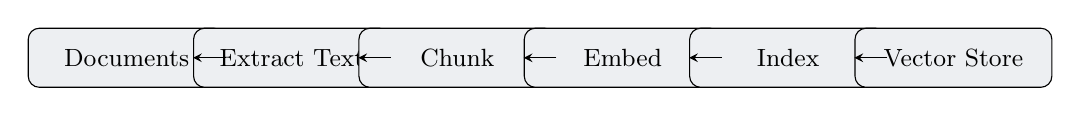
\begin{tikzpicture}[node distance=1.6cm,>=stealth,font=\small,
  box/.style={draw,rounded corners,fill=navy!8,minimum width=2.5cm,minimum height=0.75cm,align=center}]
  \node[box] (docs) {Documents};
  \node[box,right of=docs,xshift=0.5cm] (extract) {Extract Text};
  \node[box,right of=extract,xshift=0.5cm] (chunk) {Chunk};
  \node[box,right of=chunk,xshift=0.5cm] (embed) {Embed};
  \node[box,right of=embed,xshift=0.5cm] (index) {Index};
  \node[box,right of=index,xshift=0.5cm] (store) {Vector Store};
  \draw[->] (docs)--(extract); \draw[->] (extract)--(chunk);
  \draw[->] (chunk)--(embed); \draw[->] (embed)--(index); \draw[->] (index)--(store);
\end{tikzpicture}
\end{center}

\subsection{The Query Pipeline (CQRS Query Side)}

This runs for every user request, in real time.

\begin{center}
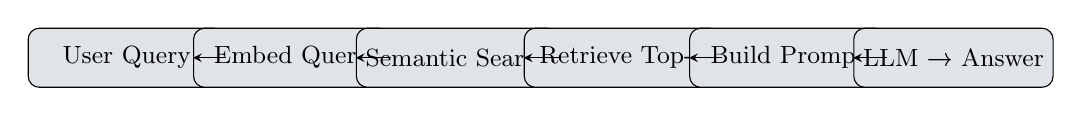
\begin{tikzpicture}[node distance=1.6cm,>=stealth,font=\small,
  box/.style={draw,rounded corners,fill=navy!14,minimum width=2.5cm,minimum height=0.75cm,align=center}]
  \node[box] (q) {User Query};
  \node[box,right of=q,xshift=0.5cm] (qe) {Embed Query};
  \node[box,right of=qe,xshift=0.5cm] (search) {Semantic Search};
  \node[box,right of=search,xshift=0.5cm] (ctx) {Retrieve Top-k};
  \node[box,right of=ctx,xshift=0.5cm] (prompt) {Build Prompt};
  \node[box,right of=prompt,xshift=0.5cm] (llm) {LLM → Answer};
  \draw[->] (q)--(qe); \draw[->] (qe)--(search); \draw[->] (search)--(ctx);
  \draw[->] (ctx)--(prompt); \draw[->] (prompt)--(llm);
\end{tikzpicture}
\end{center}

\begin{worked}{RAG query for shoe return policy}
\textbf{User query:} ``What is the return policy for shoes?'' \\[4pt]
\textbf{Step 1 --- Embed query:} Query embedded into 384-dim vector $\mathbf{q} \in \mathbb{R}^{384}$ using \texttt{all-MiniLM-L6-v2}. \\[4pt]
\textbf{Step 2 --- Semantic search:} ChromaDB computes cosine similarity between $\mathbf{q}$ and all stored chunk embeddings using the HNSW index. Top-3 results: \\
\quad Chunk 47: ``Returns accepted within 30 days for footwear...'' (similarity: 0.91) \\
\quad Chunk 12: ``Original packaging required for shoe returns...'' (similarity: 0.87) \\
\quad Chunk 83: ``Sale items, including shoes on discount, are non-returnable...'' (similarity: 0.81) \\[4pt]
\textbf{Step 3 --- Build prompt:} \\
\texttt{Context: [Chunk 47 text] [Chunk 12 text] [Chunk 83 text]\\
Question: What is the return policy for shoes?\\
Answer based only on the context above.} \\[4pt]
\textbf{Step 4 --- LLM answer:} ``Shoes can be returned within 30 days in their original packaging. Sale items are non-returnable.'' \\[4pt]
\textbf{No hallucination:} The LLM cannot invent a policy because the instruction says ``answer based only on the context.''
\end{worked}

\noindent\textbf{Vector Stores:} ChromaDB (local, open-source, SQLite + HNSW), Pinecone (managed, scalable), FAISS (Facebook, fast in-memory). \textbf{Embedding models:} OpenAI Embeddings, SBERT, DPR.

%==============================================================
\section{Monolithic Architecture}
%==============================================================

A \vocab{monolithic} application packages all its functionality into a single deployable unit. The classic example is the FTGO (Food to Go) app: Order Management, Restaurant Management, Delivery Management, Customer Management, and Payment Processing all live in one WAR file connecting to one MySQL database.

\begin{center}
\resizebox{\linewidth}{!}{%
\begin{tabular}{lll}
\toprule
\textbf{Property} & \textbf{Advantage} & \textbf{Disadvantage} \\
\midrule
Deployment & Single WAR file; simple CI/CD & Full redeploy for any change \\
Communication & In-process; fast (no network) & All modules share same failure domain \\
Scalability & One unit scales together & Cannot scale individual bottleneck components \\
Technology & One language, one framework & Technology lock-in; new tech = rewrite \\
Complexity & Easy to understand at first & Grows unmanageable as team/features grow \\
\bottomrule
\end{tabular}}
\end{center}

\begin{everyday}
A monolith is like a Swiss Army knife: one tool, convenient, always in one piece. Great for one person camping. Terrible when 50 people each need a different blade simultaneously and you can only sharpen the whole knife at once.
\end{everyday}

\noindent\textbf{Monolithic ML Pattern:} A research prototype or early-stage ML product often starts as a monolith. The web app, model loading, preprocessing, and prediction logic all live in one Flask application. Issues: updating the model requires full redeployment (risky), single point of failure, memory pressure from loading multiple large models in one process.

%==============================================================
\section{Microservices Architecture}
%==============================================================

\vocab{Microservices} decompose an application into small, independent services, each owning its own database and exposing its own API. Each service is deployable independently.

\begin{intuition}
A microservices architecture is like a food court. Each stall (pizza, sushi, tacos) is independently owned, staffed, and managed. A long queue at the pizza stall doesn't affect the sushi stall. You can renovate the taco stall without closing the whole court. Each stall uses its own kitchen equipment.
\end{intuition}

The underlying principle is Robert C. Martin's \vocab{Single Responsibility Principle}: \emph{``Gather together things that change for the same reason; separate things that change for different reasons.''}

\begin{worked}{Scaling cost: monolith vs microservices}
FTGO app handles 1{,}000 requests/sec normally. During lunch peak, the Order Service gets 5{,}000 requests/sec, but other services remain at baseline. \\[4pt]
\textbf{Monolith:} Must scale the entire application $5\times$. Cost: 5$\times$ compute for ALL services. \\
\textbf{Microservices:} Scale only the Order Service $5\times$. Restaurant, Delivery, Payment services stay at $1\times$. \\
\textbf{Cost ratio:} If the app has 5 equal services, monolith cost = $5 \times 5 = 25$ units. Microservices cost = $5 + 1 + 1 + 1 + 1 = 9$ units. Microservices uses \textbf{64\,\% less compute} during peak.
\end{worked}

\begin{worked}{ML microservices demo}
A fraud detection system decomposed into three services: \\[4pt]
\textbf{Gateway Service} (port 8000): Receives transaction POST requests, routes to downstream services. \\
\textbf{Model Service} (port 8001): Loads the fraud detection model, returns \texttt{\{"fraud\_probability": 0.94\}}. \\
\textbf{Logging Service} (port 8002): Receives prediction + transaction, writes to PostgreSQL for drift monitoring. \\[4pt]
Each service has its own Docker container. Updating the model (retraining with new fraud patterns) deploys only the Model Service container. The Gateway and Logging services keep running without interruption.
\end{worked}

\begin{watchout}
Microservices add distributed systems complexity: network latency, service discovery, distributed tracing, and the need for an API gateway. Start with a monolith, identify the bottleneck, and extract \emph{that one service}. Don't build microservices from day one for a two-person team.
\end{watchout}

\begin{keytake}
Microservices enable independent scaling, deployment, and technology choice per service. The trade-off is operational complexity that a monolith avoids.
\end{keytake}

\end{document}
